\section{Introducción}
\subsection{¿Qué es la visión artificial?}

Los seres humanos somos capaces de percibir con facilidad el entorno tridimensional que nos rodea. Durante décadas, el funcionamiento de nuestra visión ha sido fruto de extensivo estudio por parte de psicólogos de la percepción, pero aún no se conoce el funcionamiento de manera exacta  \cite{book:szeliski}.

Paralelamente, los investigadores en visión artificial han desarrollado técnicas matemáticas para, a partir de imágenes, reconstruir la apariencia tridimensional de objetos. Actualmente somos capaces de, entre otras cosas, generar un modelo 3D parcial de un entorno a partir de miles de fotografías solapadas, seguir el movimiento de una persona sobre un fondo complejo y, con moderado éxito, reconocer y nombrar a las personas de una fotografía a partir de características como el pelo, la cara o la ropa. Entre otras aplicaciones más avanzadas se encuentran detectar y clasificar objetos o elaborar descripciones verbales a partir de imágenes o vídeos.

Sin embargo, a pesar de estos avances, hacer que un ordenador sea capaz de interpretar una imagen al mismo nivel que lo haría un niño sigue siendo un sueño sin cumplir. La dificultad del problema que nos ocupa suele ser subestimada, ya que se suele tender a pensar que las partes difíciles de la inteligencia artificial son las cognitivas y no las relativas a la percepción.

Pero, ¿qué es lo que hace tan difícil la visión por computador? En parte es que, dado nuestro desconocimiento del funcionamiento de nuestra visión, es un \textit{problema inverso}: dada una cantidad insuficiente de información (una imagen o un video), tratamos de llegar a las incógnitas que nos permiten especificar una solución completa. Es decir, a partir de una imagen, tratamos de reconstruir no sólo las propiedades de los objetos que allí aparecen (como su forma, iluminación, color o posición), sino también el reconocimiento (clasificación o etiquetado de dichos objetos), la separación del resto de la escena (segmentación), etc.

Ahora bien, no todo son malas noticias: la visión por computador tiene numerosos casos de uso hoy en día. Entre sus aplicaciones encontramos cosas como (\citeauthor*{book:szeliski}):
\begin{itemize}
  \item \textbf{Reconocimiento de caracteres óptico.} Se ha llegado a reconocer caracteres numéricos con una tasa de error del 0.23\% \cite{art:2012arXiv1202.2745C}.
  \item \textbf{Inspección mecanizada.} Inspección de partes de automóviles o aeronaves a fin de, por ejemplo, encontrar defectos en el metal (Figura \ref{fig:apps1a}).
  \item \textbf{Construcción de modelos 3D.} Construcción automatizada de modelos 3D a partir de fotografías aéreas como las que usa Google
        (Figura \ref{fig:apps1b}).
  \item \textbf{Seguridad en automóviles.} Reconocimiento de obstáculos tales como peatones u otros coches, en condiciones en las que el radar o el lídar no funcionan bien, en tecnologías como \href{https://www.mobileye.com/}{Mobileye}.
  \item \textbf{Reconocimiento de huellas dactilares y biométricas.} Usado ampliamente hoy en día en teléfonos móviles.
  \item \textbf{Reconocimiento y localización de objetos, categorías y acciones.} Usando deep learning, se ha conseguido un cierto grado de precisión a la hora de reconocer objetos dispersos en una escena.
\end{itemize}

\begin{figure}
  \begin{subfigure}{.5\textwidth}
    \centering
    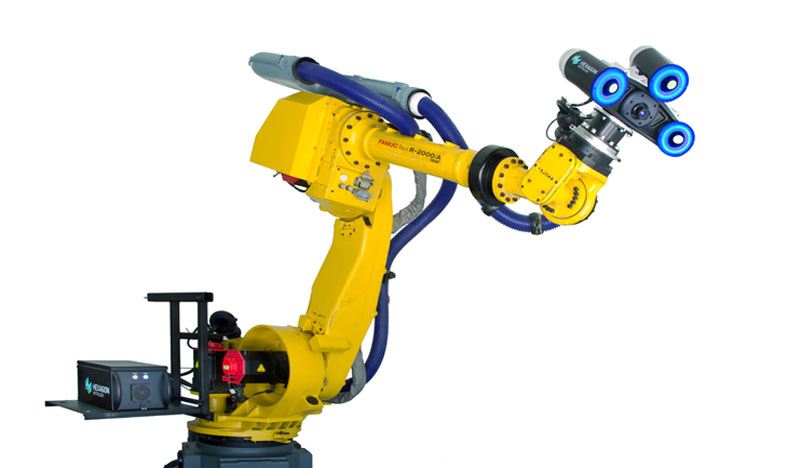
\includegraphics[width=.9\linewidth]{images/camera.jpg}
    \caption { }
    \label{fig:apps1a}
  \end{subfigure}%
  \begin{subfigure}{.5\textwidth}
    \centering
    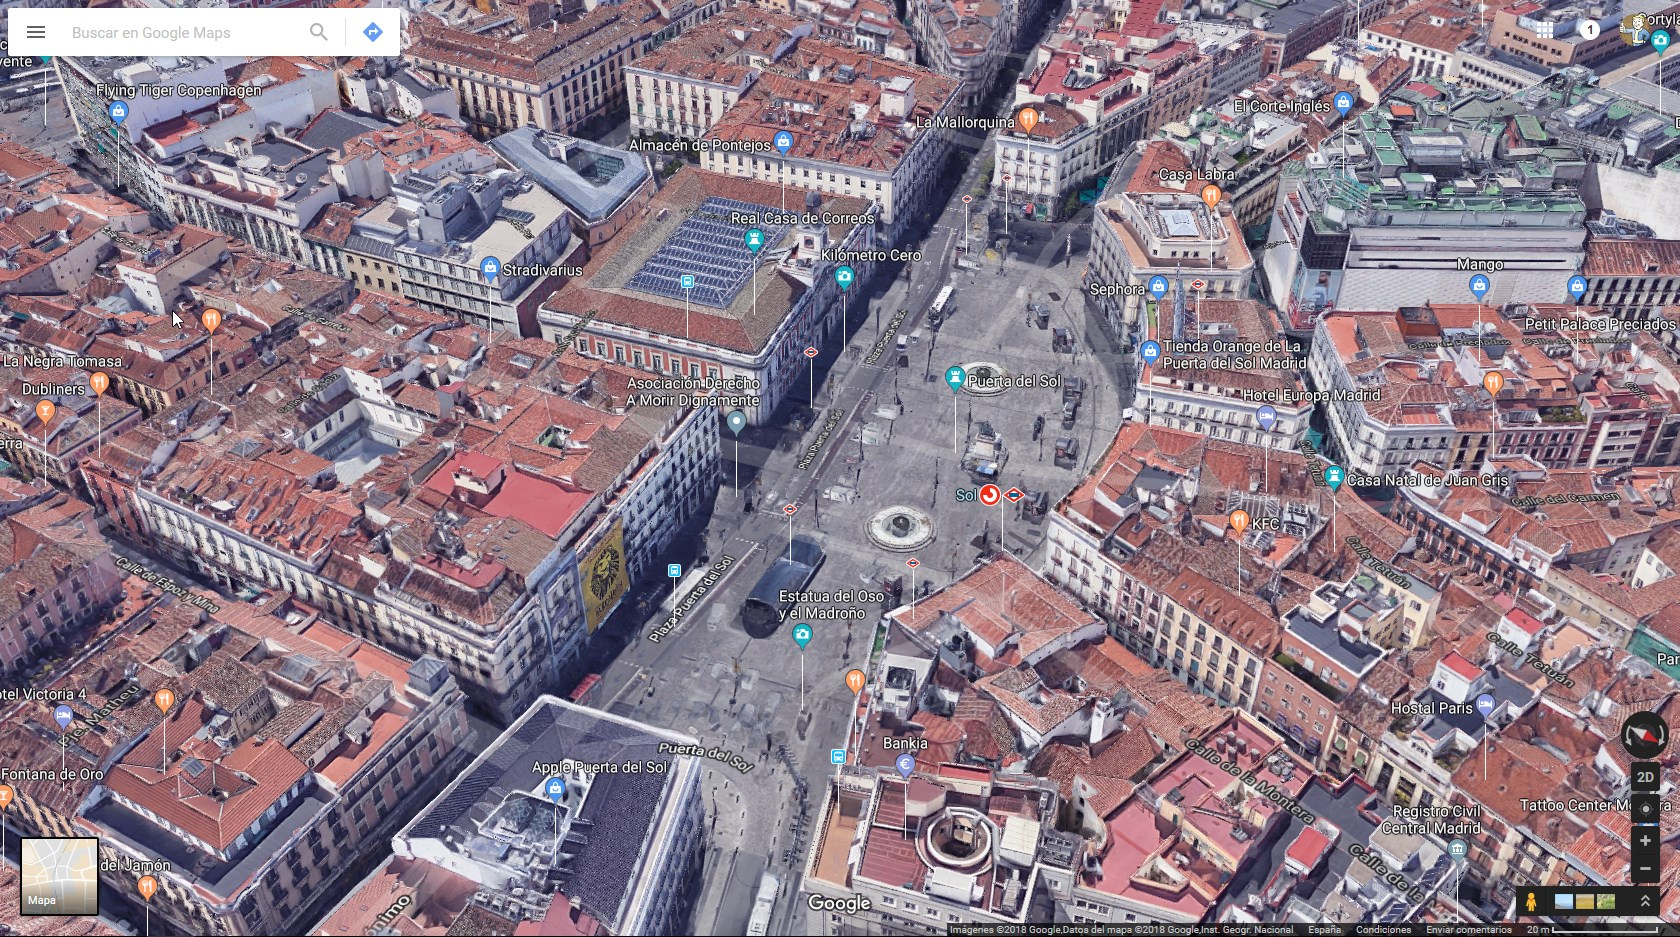
\includegraphics[width=.9\linewidth]{images/maps.jpg}
    \caption { }
    \label{fig:apps1b}
  \end{subfigure}
  \caption{Algunas aplicaciones de la visión artificial: (a) sistema de digitalizado por luz blanca \href{http://www.hexagonmi.com/es-ES/products/white-light-scanner-systems/hexagon-metrology-wls400a}{WLS400A}. (b) reconstrucción 3D en Google Maps de la Puerta del Sol. }
  \label{fig:applications}
\end{figure}

\subsection{Breve historia de la visión artificial}

\begin{figure}[H]
  \centering
  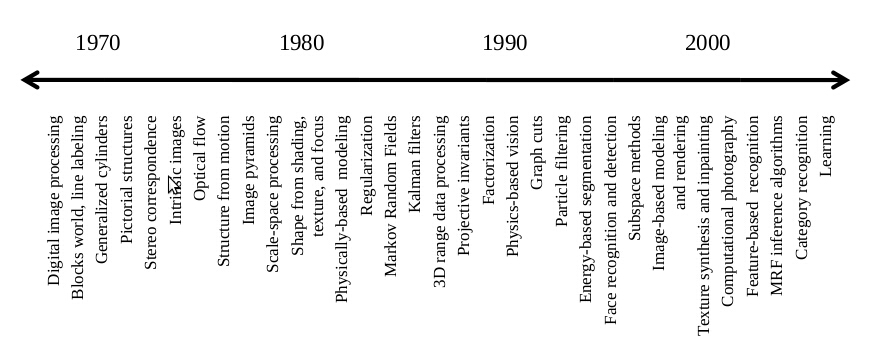
\includegraphics[width=0.8\textwidth]{images/timeline}
  \caption{Timeline de las aportaciones más importantes a la visión artificial \cite{book:szeliski}.}
\end{figure}

La investigación en visión artificial comienza en la \textbf{década de los 70}. En esta época, los pioneros en el campo de la IA y la robótica creían que resolver el problema de la entrada visual sería un trabajo fácil hacia la resolución de problemas de mayor envergadura. De hecho, tanto es así, que en 1966 Marvin Minsky le asignó a su alumno en el MIT Gerald Jay Sussman un proyecto de verano que consistía en enlazar una cámara a un ordenador y que este describiera lo que veía.

Lo que distinguió la visión por computador del campo del procesado de imágenes digitales fue la intención de reconstruir la estructura tridimensional del mundo a partir de las imágenes. Los primeros intentos en este sentido estaban relacionados con la extracción de ejes y posterior inferencia de la estructura 3D del objeto.

En la \textbf{década de 1980} los esfuerzos se centraron en técnicas matemáticas mas sofisticadas para el análisis. Empiezan a usarse ampliamente técnicas como las pirámides de imágenes, y continuó la investigación en una mejor detección de bordes y contornos. Comienzan a adoptarse técnicas de detección de formas a partir de sombreado, textura, o enfoque. Posteriormente, algunos investigadores vieron que estas técnicas podían ser generalizadas usando el mismo modelo matemático si se planteaban como problemas de optimización. También aparecieron las primeras redes neuronales aplicadas al campo de la visión por computador.

En la \textbf{década de 1990} continuó la investigación en todo lo anteriormente mencionado, pero algunos de los temas vieron un aumento en su actividad. Hubo un esfuerzo por solucionar el problema de la estructura a partir del movimiento. El trabajo comenzado en la década anterior consistente en usar medidas detalladas de color e intensidad en combinación con modelos físicos precisos acabó por crear su propio subcampo llamado visión basada en la física.

Los algoritmos de \textit{tracking} mejoraron, incluidos los de tracking por contorno usando contornos activos, así como los basados en intensidad. Normalmente se aplicaron al seguimiento de caras o de cuerpos completos.

La segmentación de imagen fue un tema de investigación activo, y surgen técnicas como \textit{mean shift}. Comienzan a aparecer técnicas de aprendizaje basadas en la estadística, de las que surgen los primeros algoritmos de reconocimiento facial.

El avance más notable en esta década fue la interacción con la computación gráfica. La idea de manipular imágenes del mundo real para crear animaciones tomó forma mediante técnicas de \textit{morphing} y se aplicó después a técnicas de
y creación de imágenes panorámicas. A la vez, empezaron a introducirse técnicas consistentes en crear modelos 3D a partir de colecciones de imágenes.

Durante la \textbf{década de los 2000} continuó la interacción entre el campo de la visión y el de los gráficos. Una tendencia de esta década fue la proliferación de técnicas basadas en \textit{features} para el reconocimiento de objetos. Estas técnicas también dominan otras tareas del reconocimiento como el reconocimiento de la escena o de localización.

Otra tendencia, que sigue presente en la actualidad, es la aplicación de técnicas de \textit{machine learning} a problemas de visión artificial, como es el uso de redes neuronales convolucionales. El crecimiento de esta técnica coincide con la gran disponibilidad en Internet de enormes cantidades de datos etiquetados, así como la multiplicación de la capacidad de cómputo, lo que facilitó las tareas de aprendizaje.

Al igual que en el campo del \textit{machine learning}, las redes neuronales han cobrado una importancia vital, y se ha logrado avances verdaderamente grandes haciendo uso de ellas. Un ejemplo del estado actual del campo es el trabajo de \citet{art:2017arXiv170306870H} que muestra el avance en segmentación de imagen que se ha logrado usando ANN (\textit{Artificial Neural Network}).

También hay avances en la conducción autónoma usando visión por computador, de hecho NVIDIA tiene actualmente en funcionamiento una plataforma para coches autónomos llamada NVIDIA DRIVE. Dicha plataforma, nuevamente, hace uso de técnicas de deep learning para detectar obstáculos, señales, etc.

\subsection{El \textit{deep learning} y su aportación a la visión artificial}
\subsubsection*{Orígenes de las ANN}

El término \textit{deep learning} se refiere al conjunto de técnicas basadas en redes neuronales que permiten a un ordenador aprender a resolver una tarea concreta mediante el aprendizaje automático. En esencia, es una forma de \textit{machine learning}. Dichas redes neuronales, permiten crear modelos capaces de extraer \textit{features} abstractas de alto nivel, como pueden ser caras, voces o coches, a partir de conceptos más sencillos como el color, los contornos o las esquinas (\citet{book:Goodfellow-et-al-2016}).

El concepto de red neuronal no es en absoluto novedoso, ya en 1943 el neurólogo Warren McCulloch y el matemático Walter Pitts las propusieron en un artículo \cite{art:mcculloch1943logical} en el que se presentaba un modelo computacional de cómo las neuronas biológicas funcionaban en conjunto para realizar cálculos complejos utilizando lógica proposicional.

Los éxitos iniciales de las ANN llevaron a la creencia de que la IA era inminente. Sin embargo, en los años 60 se vio que esto no iba a ocurrir pronto, así que las ANN quedaron en espera hasta los años 80, cuando se desarrollaron nuevas arquitecturas y técnicas de entrenamiento que llevaron a revivir el interés. En los años 90 se propusieron técnicas de machine learning como las máquinas de soporte vectorial (SVM), las cuales ofrecían mejores resultados (y más comprensibles) que las redes neuronales, así que volvieron a caer en el olvido.

En las dos últimas décadas ha habido una nueva oleada de interés por las redes neuronales, la cual parece diferente a las anteriores en cuanto a las circunstancias en las que se produce (actualmente tenemos una cantidad de datos ingente, mejor capacidad de procesamiento y mejores algoritmos de entrenamiento), así que podría ser la definitiva \cite{book:homl}.

El ejemplo más típico de un modelo \textit{deep learning} es el perceptrón multicapa (MLP, figura \ref{fig:mlp}), el cual consiste en una serie de ``neuronas'' conectadas entre sí a través de una o más capas. Cada una de dichas neuronas, en realidad es una función matemática que en la última capa produce una salida, la cual se utiliza en un proceso denominado \textit{backpropagation}. El objetivo del proceso es reajustar los pesos de cada uno de los perceptrones o neuronas que se hallan en el modelo, de forma que se reduzca el error en sucesivas iteraciones. Este algoritmo se propuso en 1987 \cite{art:backpropagation} y sigue siendo utilizado hoy en día.

\begin{figure}[H]
  \centering
  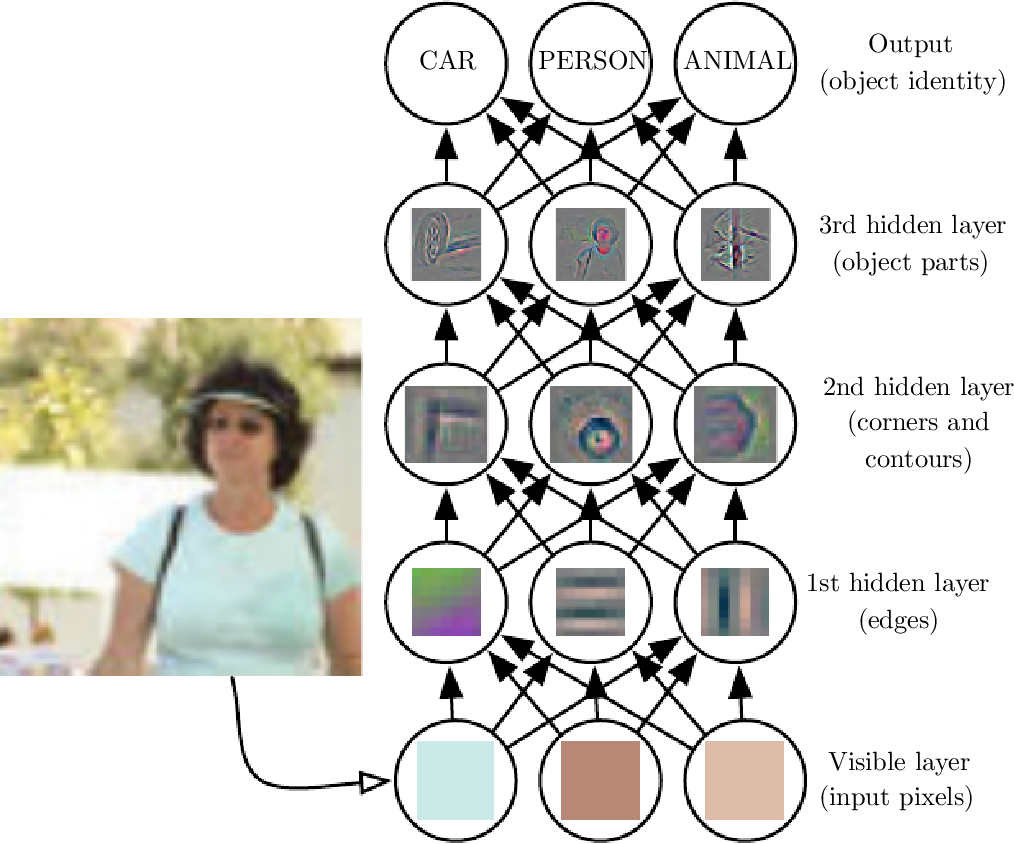
\includegraphics[width=0.6\textwidth]{images/mlp}
  \caption{Esquema de funcionamiento de un MLP \cite{book:Goodfellow-et-al-2016}.}
  \label{fig:mlp}
\end{figure}

\subsubsection*{Uso de las redes neuronales convolucionales para visión computacional}

\begin{figure}[H]
  \centering
  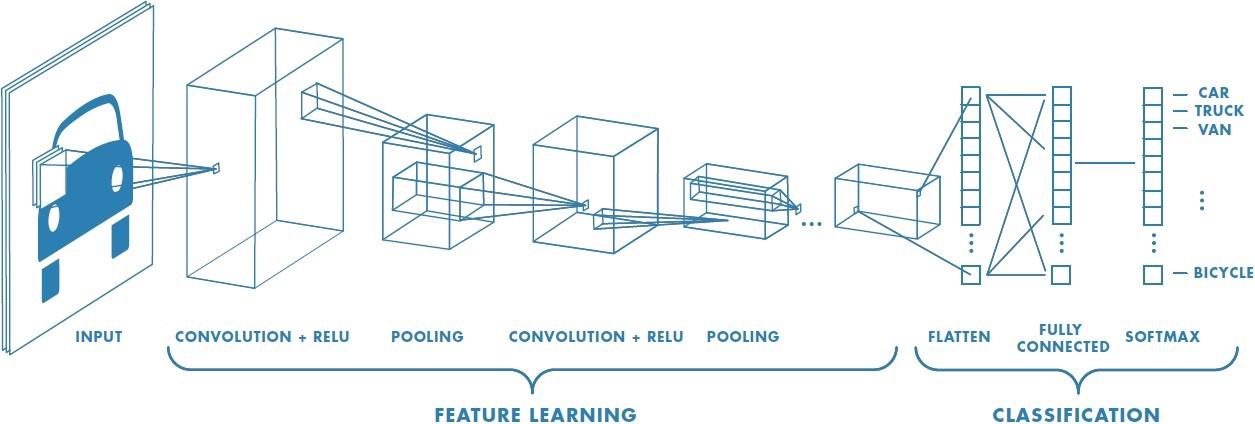
\includegraphics[width=0.6\textwidth]{images/cnn}
  \caption{Esquema de funcionamiento de una CNN.}
  \label{fig:cnn}
\end{figure}

En 1958 \cite{art:cat58} y 1959 \cite{art:cat59}, David H. Hubel y Torsten Wiesel llevaron a cabo una serie de experimentos sobre el córtex visual de los gatos. En ellos, se halló la cantidad de neuronas que se encuentran en dicho córtex y cómo este funcionaba: se vio que las neuronas del córtex tienen un pequeño campo receptivo sobre todo el campo visual y la combinación de todos los campos receptivos es el campo visual total. Además, algunas neuronas reaccionaban a imágenes de líneas horizontales y otras a líneas verticales, mientras que otras neuronas tenían un campo receptivo mayor, de forma que combinaban estos patrones de bajo nivel en otros más complejos.

Estos estudios inspiraron la creación del neocognitron \cite{art:neocognitron}. Esto modelo fue evolucionando hasta convertirse en lo que hoy conocemos como redes neuronales convolucionales. Un hito fue el artículo de \citet{lecun1998gradient} donde se propuso la arquitectura LeNet-5, utilizada por bancos para reconocer números escritos sobre cheques. La diferencia de las redes neuronales convolucionales sobre las clásicas es el empleo de capas convolucionales y de pooling. Típicamente, al final de las capas ocultas, se emplean capas densamente conectadas hasta llegar a la capa final donde se da la salida \cite{book:homl}.

La irrupción de las CNN junto con la mayor capacidad de procesamiento matricial (principalmente en GPUs), ha propiciado resultados muy buenos en diversos ámbitos, entre ellos el de la visión artificial, donde son utilizadas como la arquitectura más utilizada en problemas de este tipo, ya que tienden a dar mejores resultados en problemas complejos que otros modelos más clásicos. De hecho, las redes tipo CNN han demostrado rendimiento mejor que el humano en ciertos problemas de reconocimiento visual.

Incluso, se plantea un debate sobre si las técnicas clásicas de visión computacional están obsoletas en favor de las redes neuronales convolucionales en trabajos como \cite{art:o2019deep}, aunque en ciertos dominios siguen siendo utilizadas dichas técnicas (a veces en conjunto a las CNN).

Un tipo particular de CNN son las que no cuentan con ninguna capa densa dentro de su arquitectura, denominadas \textit{fully convolutional network} o FCN y que fueron propuestas en 2015 (\citet{art:FCN2015}) para problemas de segmentación semántica. La ventaja de este tipo de arquitectura es que no requiere que las imágenes tengan un tamaño fijo, mientras que las CNN con capas densas requieren un tamaño concreto que coincide con el tamaño de las imágenes de entrenamiento. Una arquitectura de este tipo es la YOLO (\textit{you only look once}), propuesta en 2015 \cite{art:yolo} y mejorada en sucesivos trabajos en 2016 \cite{art:yolo2} y 2018 \cite{art:yolo3}.

\begin{figure}
  \centering
  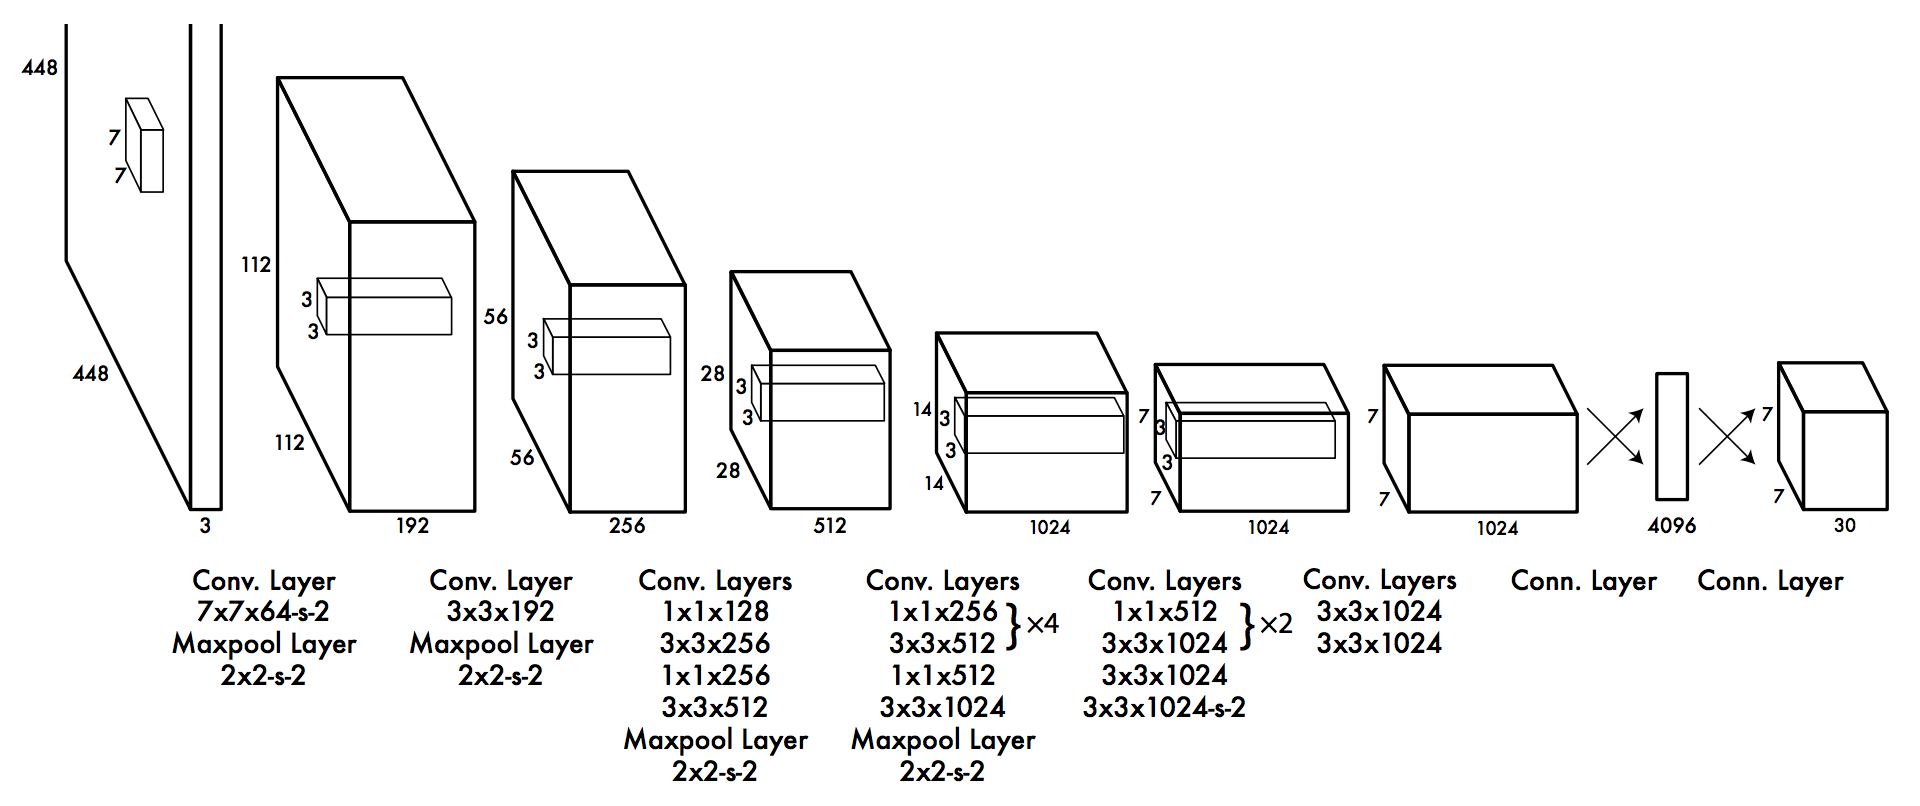
\includegraphics[width=0.8\textwidth]{images/yolo.png}
  \caption{Estructura de red del modelo YOLO \cite{art:yolo}.}
  \label{fig:yoloArch}
\end{figure}

\newpage